\section{Lecture 5}
\begin{itemize}
    \item There is a linear relationship between the force of a wire and the deformation. The slope was called the stiffness:
    \begin{equation}
        k = \frac{F}{\Delta L}
        \label{eq:}
    \end{equation}
    The problem with this is that the slope would be different for different sizes of the same object, so it didn't reflect a particular object's characteristics.
    \item Young modified this relationship to instead measure the tensile strength $\sigma=F/A$ in terms of the strain $\epsilon=\frac{\Delta L}{L}$, such that:
    \begin{equation}
        E = \frac{\sigma}{\epsilon}
        \label{eq:}
    \end{equation}
    This provides a method to experimentally determine the value of $E$, by loading different weights and measuring the strain for each.
    \item A \textbf{Coupon Test} is the testing of a small representative piece of a material to determine the properties. We do this via the setup below, where we place two indicators a length $L_0$ apart. As we load weight onto the rectangle, the distance between the indicators will change to $L_0+\Delta L$.
    \begin{center}
        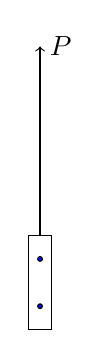
\begin{tikzpicture}[scale=0.3]
            \draw[] (-0.5,2) rectangle (0.5,-2);
            \draw[fill=blue] (0,1) circle (0.1);
            \draw[fill=blue] (0,-1) circle (0.1);
            \draw[->] (0,2) -- (0,10) node[right] {$P$};
        \end{tikzpicture}
    \end{center}
    \item We can increase the strain by adding weights below and measuring the force $P$. Dividing it through by the area gives the tensile strength.
    \begin{center}
        \begin{tikzpicture}
            \coordinate (O) at (0,0);
            \draw[->] (O) -- (12,0) node[above] {$\epsilon$};
            \draw[->] (O) -- (0,6);
            
            \draw[<->,dotted] (0,2.5) -- (3,2.5) node[midway,above] {$\text{linear elastic}$};
            \draw[] (O) -- (3,2);

            \draw[<->, dotted] (3,2.5) -- (6,2.5) node[midway,above] {$\text{yield plateau}$};
            \draw[] (3,2) -- (6,2);
            \draw[dotted] (3,2) -- (0,2) node[left] {$\sigma_{yield}$};
            \draw (0,4) node[left] {$\sigma_{ultimate}$};

            \draw[] (9,4) parabola (6,2);
            \draw[<->, dotted] (6,2.5) -- (9,2.5) node[midway,above] {$\text{strain hardening}$};
            \draw[] (9,4) parabola (11,3);
            \draw[<->, dotted] (9,2.5) -- (11,2.5) node[midway,above] {$\text{necking}$};

        \end{tikzpicture}
    \end{center}
    \item The \textbf{yield plateau} occurs when the atoms in the metal are no longer vibrating back and forth between one another, but sliding across one another. As a result, we experience \textbf{permanent plastic deformations} during this period.
    \item At a certain point, the imperfections build up such that yielding becomes more difficult, so in order to overcome them, the stress increases. This process is known as \textbf{strain hardening}.
    \item \textbf{Necking} occurs after the ultimate stress point where the cable will form a neck shape, reducing the tensile strength.
    \item \textbf{Rupture} occurs after the cable cannot support the strain at all and then break.
    \item If the applied load is taken off, the cable will contract back to $\sigma=0$ following the same slope. After the initial yield plateau, the cable will not be able to naturally go back to its original rest length.
\end{itemize}